\subsection{Coil}
\label{Coil problems}
Since the scope of the project was the validation of the converter, it was decided to implement an existing inductor. A coil was then selected with an approximate inductance of slightly over $1mH$.
The PCB was then designed for this initial inductor. However, after some  tests under high currents it was shown that the coil was not maintaining its inductance due to saturation of the core. Also, it was reaching temperatures over $100\dec C$. The inductance was then tested under different currents and the behavior was verified as shown in figure \ref{Coil comparison}.

It was then decided to implement another inductor which would satisfy the requirements in all cases. The same tests were performed for the new inductor and it was shown that it would fulfill the requirements without problems. 
Also, some thermal tests were performed on the new inductor. With a constant current of $10A$, it shows a maximum temperature of $60\dec C$ after 10 minutes.

\begin{figure}[H]
	\begin{center}
		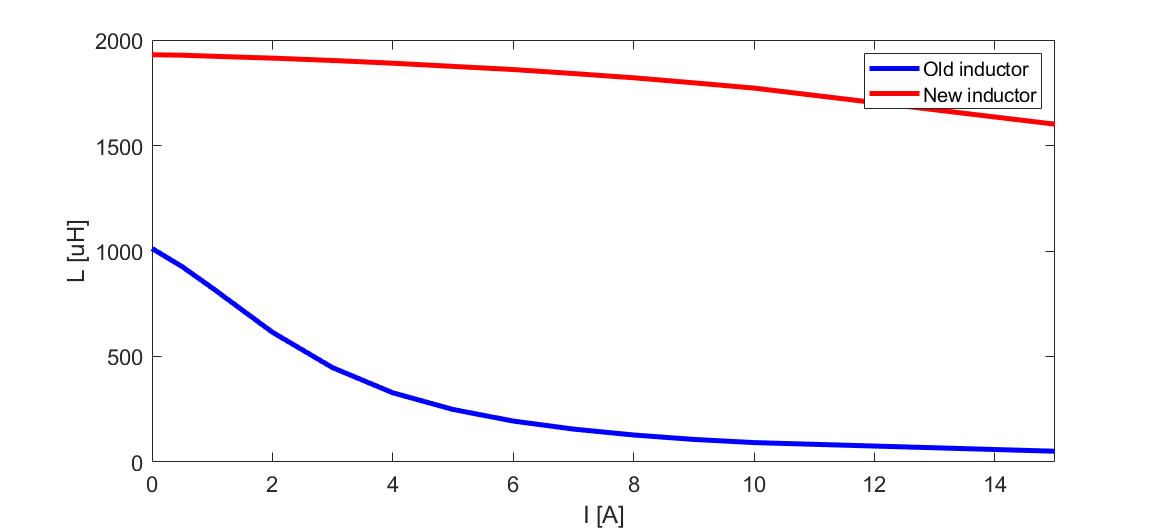
\includegraphics[width=1\textwidth]{docs/discussion/CoilTests/CoilComparison50kHzV2.png}
		\caption{Inductor comparison under changes on current flow (50kHz).}
		\label{Coil comparison}
	\end{center}	
\end{figure}

However, the size and weight of the new inductor are much higher than those of the previous one. This means that the footprint designed is not valid for the new coil and it hangs loose outside the PCB.